\section{Introduction}

\subsection{Overview}

The NUbots from the University of Newcastle, Australia have had a strong record of success in the RoboCup Four Legged League since first entering in 2002. The Nubots achieved 3rd place in 2002 (Fukuoka), and again in 2003 (Padua) and 2004 (Lisbon). In 2005 (Osaka) with a complete redevelopment of the code, the NUbots came 2nd in a heartbreaking penalty shoot out against the German Team. With a strong 2005 base code, 2006 development focused on debugging and fine tuning. The result was a nail biting final against rUNSWift in Bremen where the NUbots won 7-3. Code development plateaued in 2007 and we lost the final in Atlanta against the Northern Bites, a relatively new team who was heavily influenced by our methods.  

2008 was a year of change. The transition from the Sony ERS-7 robot to the Aldebaran Nao meant a total rewrite of the software system. In addition, two of our main team members left. Michael Quinlan was `poached' by UT Austin and Rick Middleton moved to the National University of Ireland, Maynooth (NUIM). With a limited number of places available in the new Nao League we decided to collaborate with Rick and NUIM to form a joint team, the `NUManoids'. 

2008 was also a year of challenges. University payment issues, splitting the robot package and repair delays meant even that we had even less time to work on the robot than originally planned. But with all these changes and challenges, we successfully over came them to become first world champions of the Robocup Nao SPL. 

This year was another year of change, where we decided to separate from NUIM and once again become the NUbots. With only half the original team size (only four active members), we set out to improve the previous years code. With major improvements to vision, localisation and locomotion it was not enough to defend our title from the much larger teams in the competition. Due to this, we completed the competition with a ranking of quarter finalist.

This report will outline the system and some more recent advances added into the system this year.

\subsection{Software Layout}

Our 2009 system was based on last years architecture \cite{NUManoids2008}which originated from the Sony Aibo architecture in 2006 \cite{NUBOT2006}. Our system consists of one control module \emph{Nao} and four functional modules -
\emph{Vision, Localisation, Behaviour and Locomotion}. 

The flow of information in our system can be seen in Figure
\ref{fig:software}. 

\begin{figure}[!h]
\begin{center}
    %\leavevmode
    \scalebox{0.5} {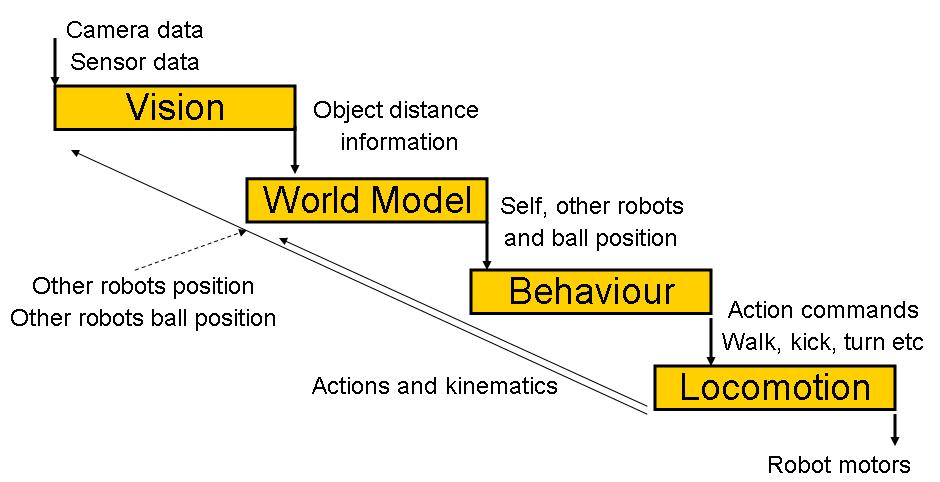
\includegraphics{figs/software.jpg} }
    \caption{2009 Software Architecture}
    \label{fig:software}
\end{center}
\end{figure}

